%%%%%%%%%%%%%%%%%%%%%%%%%%%%%%%%%%%%%%%%%%%%%%%%%%%%%%%%%%%%%%%%%%%%%%%%%%%%%%%
%% Descr:       Vorlage für Berichte der DHBW-Karlsruhe
%% Author:      Prof. Dr. Jürgen Vollmer, vollmer@dhbw-karlsruhe.de
%% $Id: bericht.tex,v 1.19 2016/03/16 16:59:41 vollmer Exp $
%%  -*- coding: utf-8 -*-
%%%%%%%%%%%%%%%%%%%%%%%%%%%%%%%%%%%%%%%%%%%%%%%%%%%%%%%%%%%%%%%%%%%%%%%%%%%%%%%

\documentclass[
   ngerman          % neue deutsche Rechtschreibung
  ,a4paper          % Papiergrösse
% ,twoside          % Zweiseitiger Druck (rechts/links)
% ,10pt             % Schriftgrösse
% ,11pt
  ,12pt
  ,pdftex
%  ,disable         % Todo-Markierungen auschalten
]{report}

% Bitte die Codierung Ihrer Dateien auswählen:
% \usepackage[latin1]{inputenc}    % Für UNIX mit ISO-LATIN-codierten Dateien
% \usepackage[applemac]{inputenc}  % Für Apple Mac
% \usepackage[ansinew]{inputenc}   % Für Microsoft Windows
  \usepackage[utf8]{inputenc}        % UTF-8 codierte Dateien
                                   % Dieses Dokument ist unter Unix erstellt, daher
                                   % wird diese Input-Codierung benutzt.

\usepackage{bericht}
\usepackage{setspace}
\usepackage{listings}

%%%%%%%%%%%%%%%%%%%%%%%%%%%%%%%%%%%%%%%%%%%%%%%%%%%%%%%%%%%%%%%%%%%%%%%%%%%%%%%
%% Angaben zur Arbeit
%%%%%%%%%%%%%%%%%%%%%%%%%%%%%%%%%%%%%%%%%%%%%%%%%%%%%%%%%%%%%%%%%%%%%%%%%%%%%%%

\newcommand{\Autor}{Patrick Siewert}
\newcommand{\MatrikelNummer}{4363889}
\newcommand{\Kursbezeichnung}{TINF16B2}

\newcommand{\FirmenName}{Fiducia \& GAD IT AG}
\newcommand{\FirmenStadt}{Karlsruhe}
\newcommand{\FirmenLogoDeckblatt}{
\includegraphics{fiducia-gad-logo}}

% Falls es kein Firmenlogo gibt:
%  \newcommand{\FirmenLogoDeckblatt}{}

\newcommand{\BetreuerFirma}{Volker Werling}
\newcommand{\BetreuerDHBW}{Prof. Dr. Heinrich Braun}

%%%%%%%%%%%%%%%%%%%%%%%%%%%%%%%%%%%%%%%%%%%%%%%%%%%%%%%%%%%%%%%%%%%%%%%%%%%%%%%%%%%%%

\newcommand{\Was}{Projektarbeit}
% Wird auf dem Deckblatt in der Erklärung benutzt

%%%%%%%%%%%%%%%%%%%%%%%%%%%%%%%%%%%%%%%%%%%%%%%%%%%%%%%%%%%%%%%%%%%%%%%%%%%%%%%%%%%%%

\newcommand{\Titel}{Präsentation von PowerPoint-Folien durch einen Humanoiden
Roboter}
\newcommand{\AbgabeDatum}{3. April 2018}

\newcommand{\Dauer}{11 Wochen}

% \newcommand{\Abschluss}{Bachelor of Engineering}
\newcommand{\Abschluss}{Bachelor of Science}

% \newcommand{\Studiengang}{Informationstechnik}
\newcommand{\Studiengang}{Angewandte Informatik}

\hypersetup{%%
  pdfauthor={\Autor},
  pdftitle={\Titel},
  pdfsubject={\Was}
}

%%%%%%%%%%%%%%%%%%%%%%%%%%%%%%%%%%%%%%%%%%%%%%%%%%%%%%%%%%%%%%%%%%%%%%%%%%%%%%%

% Benutzt man das "biblatex"-Paket, dann muß das hier stehen:
% siehe auch die mit BIBLATEX markierten Zeilen in bericht.sty
\bibliography{bericht}

\begin{document}
\pagenumbering{roman}

%%%%%%%%%%%%%%%%%%%%%%%%%%%%%%%%%%%%%%%%%%%%%%%%%%%%%%%%%%%%%%%%%%%%%%%%%%%%%%%

\begin{titlepage}
\begin{center}
\vspace*{-2cm}
\FirmenLogoDeckblatt\hfill
\includegraphics[width=4cm]{dhbw-logo}\\[2cm]
{\Huge \Titel}\\[2cm]
{\Huge\scshape \Was}\\[2cm]
{\large für die Prüfung zum}\\[0.5cm]
{\Large \Abschluss}\\[0.5cm]
{\large des Studienganges \Studiengang}\\[0.5cm]
{\large an der}\\[0.5cm]
{\large Dualen Hochschule Baden-Württemberg Karlsruhe}\\[0.5cm]
{\large von}\\[0.5cm]
{\large\bfseries \Autor}\\[1cm]
{\large Abgabedatum \AbgabeDatum}
\vfill
\end{center}
\begin{tabular}{l@{\hspace{2cm}}l}
Bearbeitungszeitraum	         & \Dauer 			\\
Matrikelnummer	                 & \MatrikelNummer		\\
Kurs			         & \Kursbezeichnung		\\
Ausbildungsfirma	         & \FirmenName			\\
			         & \FirmenStadt			\\
Betreuer der Ausbildungsfirma	 & \BetreuerFirma		\\
Gutachter der Studienakademie	 & \BetreuerDHBW		\\
\end{tabular}
\end{titlepage}

%%%%%%%%%%%%%%%%%%%%%%%%%%%%%%%%%%%%%%%%%%%%%%%%%%%%%%%%%%%%%%%%%%%%%%%%%%%%%%%

% Nur f�r Bachelorarbeiten einf�gen:
%%%%%%%%%%%%%%%%%%%%%%%%%%%%%%%%%%%%%%%%%%%%%%%%%%%%%%%%%%%%%%%%%%%%%%%%%%%%%%%
%% Descr:       Vorlage für Berichte der DHBW-Karlsruhe, Erklärung
%% Author:      Prof. Dr. Jürgen Vollmer, vollmer@dhbw-karlsruhe.de
%% $Id: erklaerung.tex,v 1.6 2016/03/16 12:51:09 vollmer Exp $
%% -*- coding: utf-8 -*-
%%%%%%%%%%%%%%%%%%%%%%%%%%%%%%%%%%%%%%%%%%%%%%%%%%%%%%%%%%%%%%%%%%%%%%%%%%%%%%%

% In Bachelorarbeiten muss eine schriftliche Erklärung abgegeben werden.
% Hierin bestätigen die Studierenden, dass die Bachelorarbeit, etc.
% selbständig verfasst und sämtliche Quellen und Hilfsmittel angegeben sind. Diese Erklärung
% bildet das zweite Blatt der Arbeit. Der Text dieser Erklärung muss auf einer separaten Seite
% wie unten angegeben lauten.

\newpage
\thispagestyle{empty}
\begin{framed}
\begin{center}
\Large\bfseries Erklärung
\end{center}
\medskip
\noindent
Ich versichere hiermit, dass ich meine \Was\ mit
dem Thema: \enquote{\Titel} selbstständig verfasst und keine anderen als die
angegebenen Quellen und Hilfsmittel benutzt habe. Ich versichere zudem, dass die eingereichte elektronische Fassung mit der
gedruckten Fassung übereinstimmt.

\vspace{3cm}
\noindent
\underline{\hspace{4cm}}\hfill\underline{\hspace{6cm}}\\
Ort~~~~~Datum\hfill Unterschrift\hspace{4cm}
\end{framed}

\vfill
\emph{Sofern von der Ausbildungsstätte ein Sperrvermerk gewünscht wird, ist folgende Formulierung
zu verwenden:}
\begin{framed}
\begin{center}
\Large\bfseries Sperrvermerk
\end{center}
\medskip
\noindent
Der Inhalt dieser Arbeit darf weder als Ganzes noch in Auszügen Personen
auerhalb des Prüfungsprozesses und des Evaluationsverfahrens zugänglich gemacht
werden, sofern keine anders lautende Genehmigung der Ausbildungsstätte vorliegt.
\end{framed}

%%%%%%%%%%%%%%%%%%%%%%%%%%%%%%%%%%%%%%%%%%%%%%%%%%%%%%%%%%%%%%%%%%%%%%%%%%%%%%%
\endinput
%%%%%%%%%%%%%%%%%%%%%%%%%%%%%%%%%%%%%%%%%%%%%%%%%%%%%%%%%%%%%%%%%%%%%%%%%%%%%%%


\newpage
\tableofcontents           % Inhaltsverzeichnis hier ausgeben
\newpage
\listoffigures             % Liste der Abbildungen
\newpage
\listoftables              % Liste der Tabellen
\newpage
\lstlistoflistings         % Liste der Listings
\newpage
\listofequations           % Liste der Formeln

% Jetzt kommt der "eigentliche" Text
\newpage
%%%%%%%%%%%%%%%%%%%%%%%%%%%%%%%%%%%%%%%%%%%%%%%%%%%%%%%%%%%%%%%%%%%%%%%%%%%%%%
%% Descr:       Vorlage für Berichte der DHBW-Karlsruhe, Datei mit Abkürzungen
%% Author:      Prof. Dr. Jürgen Vollmer, vollmer@dhbw-karlsruhe.de
%% $Id: abk.tex,v 1.3 2016/03/16 12:21:40 vollmer draft $
%% -*- coding: utf-8 -*-
%%%%%%%%%%%%%%%%%%%%%%%%%%%%%%%%%%%%%%%%%%%%%%%%%%%%%%%%%%%%%%%%%%%%%%%%%%%%%%%

\chapter*{Abkürzungsverzeichnis}                   % chapter*{..} -->   keine Nummer, kein "Kapitel"
						         % Nicht ins Inhaltsverzeichnis
% \addcontentsline{toc}{chapter}{Akürzungsverzeichnis}   % Damit das doch ins Inhaltsverzeichnis kommt

% Hier werden die Abkürzungen definiert
\begin{acronym}[DHBW]
  % \acro{Name}{Darstellung der Abkürzung}{Langform der Abkürzung}
 \acro{Abk}[Abk.]{Abkürzung}

 % Folgendes benutzen, wenn der Plural einer Abk. benöigt wird
 % \newacroplural{Name}{Darstellung der Abkürzung}{Langform der Abkürzung}
 \newacroplural{Abk}[Abk-en]{Abkürzungen}

 \acro{H2O}[\ensuremath{H_2O}]{Di-Hydrog-Monoxid}

 % Wenn neicht benutzt, erscheint diese Abk. nicht in der Liste
 \acro{NUA}{Not Used Acronym}
 
 \acro{hri}[HRI]{Human-Robot Interaction}
 \acro{mqtt}[MQTT]{Message Queuing Telemetry Transport} 
\end{acronym}              % Abk�rzungsverzeichnis
\newpage
\onehalfspacing
\pagenumbering{arabic}
\chapter{Einleitung}\label{sec:einleitung}
\section{Die Fiducia \& GAD IT AG}\label{sec:fiducia-gad}
Die Fiducia \& GAD IT AG ist der Dienstleister für Informationstechnologie der
genossenschaftlichen FinanzGruppe. Das Unternehmen beschäftigt aktuell rund
6.400 Mitarbeiter an den Verwaltungssitzen in Karlsruhe und Münster und den
Geschäftsstellen in München, Frankfurt und Berlin. Die Fiducia \& GAD
erwirtschaftet einen jährlichen Konzernumsatz von rund 1,4 Milliarden Euro.

\subparagraph{}
Kunden der Fiducia \& GAD sind alle 1.000 Volksbanken und Raiffeisenbanken in
Deutschland und die Unternehmen der genossenschaftlichen FinanzGruppe. Außerdem
gehören zahlreiche Privatbanken und Unternehmen anderer Branchen, wie z.B. der
ADAC, zum Kundenkreis der Fiducia \& GAD.

\subparagraph{}
Neben dem Betrieb der beiden Bankverfahren "`agree21"' und "`bank21"' in ihren
vier Hochsicherheitsrechenzentren, betreut die Fiducia \& GAD 173.000
Bankarbeitsplätze und verwaltet knapp 83 Millionen Kundenkonten. Außerdem stellt
die Fiducia \& GAD mit 36.000 eigenen Selbstbedienungsgeräten bundesweit eine
reibungslose Bargeldversorgung sicher. \cite{FiduciaGAD2018}

\section{Motivation}\label{sec:motivation}
Humanoide Roboter lösen bei vielen Menschen eine große Faszination aus. Obwohl
sie in Japan bereits weit verbreitet sind und mehrere Firmen immer
fortgeschrittenere entwickeln, trifft man im realen Leben nur sehr selten auf
humanoide Roboter. Die meisten Menschen kennen diese Art Roboter nur aus
Science-Fiction Filmen. Diese verbreiten ein faszinierendes, wenn auch teilweise
beängstigendes, Bild von Robotern, die den Menschen im täglichen Leben
unterstützen und dabei in Bewegung, Sprache und Aussehen einem Menschen ähneln.
Doch humanoide Roboter sind nicht mehr nur Science-Fiction. Sie haben das
Potenzial tägliche Begleiter der Menschen zu werden, wie zuletzt der Computer,
oder als noch aktuellere technische Entwicklung, das Smartphone.

\subparagraph{}
Die Fiducia \& GAD erforscht Möglichkeiten humanoide Roboter produktiv
eizusetzen. Dazu sollen sie in eigene oder für ihre Kunden bereitgestellte
Geschäftsprozesse eingebunden werden. Zu diesen Zwecken wird der Roboter Pepper
der Firma SoftBank Robotics eingesetzt.

\section{Zielsetzung}\label{sec:zielsetzung}
Momentan werden hierbei zunächst komplexere Anwendungsszenarien betrachtet,
beispielsweise eine geführte Kontoeröffnung. Diese werden im Rahmen von
Veranstaltungen auch immer wieder bei Kunden präsentiert. Hierbei ist meist die
Einbindung eigener, zur Veranstaltung passender Inhalte erwünscht. Um dieser
Anforderung und der Usergruppe zu begegnen soll die Möglichkeit der
Präsentation von PowerPoint-Folien durch den Roboter geschaffen werden.

\subparagraph{}
Ziel ist es eine Online-Plattform zu erstellen, die PowerPoint-Dateien so
umwandelt, dass die Folien auf dem Tablet des Roboters angezeigt werden können.
Zusätzlich soll Pepper die Notizen der einzelnen Folien jeweils zur
entsprechenden Folie vorlesen. Dazu wird ein Programm geschrieben, welches die
Folien zu Bildern und Text umwandelt. Außerdem wird eine App entwickelt, die auf
dem Roboter installiert wird. So kann der Roboter die umgewandelte und
bereitgestellte Präsentation vortragen.

\newpage
\chapter{Grundlagen}\label{sec:grundlagen}
\section{Python}\label{sec:python}
Anwendungen für den Roboter Pepper (Kapitel \ref{sec:pepper}) können in Python,
C++, Java, JavaScript oder ROS programmiert werden. \cite{SoftBankIII2018} Bei
den bisherigen Anwendungen wurde Python als Programmiersprache verwendet.
Deshalb wird auch für diese Anwendung als
hauptsächliche Programmiersprache verwendet. "`Python ist eine portable,
interpretative, objektorientiere Programmiersprache"' \cite{Weigend2017}. Ihre
Entwicklung wurde 1989 von Guido van Rossum begonnen. Heute wird die Entwicklung
von der nichtkommerziellen Organisation "`Python Software Foundation"'
\footnote{\url{https://www.python.org/psf/}} koordiniert.

\subparagraph{}
Das Python-Skript wird von einem Interpreter ausgeführt. Python-Skripte können
auf verschiedenen Systemplattformen (Unix, Windows, Mac OS) ausgeführt werden.
Deshalb bezeichnet man Python als portable Sprache. Zudem gilt Python-Code als
sehr gut lesbar und ein Programm kann mit weniger Code erstellt
werden als in anderen Programmiersprachen. Listing \ref{lst:python-hello-world}
zeigt ein "`Hello World"'-Programm in Python im Vergleich zu einem Java-Programm
in Listing \ref{lst:java-hello-world}, welches die gleiche Funktion umfasst.
Die aktuelle Python Version ist 3.6.
Da auf dem Roboter allerdings Python 2.7 installiert ist, wird die Anwendung mit
dieser Version entwickelt. \cite{Weigend2017}

\begin{lstlisting}[float, language=Python, frame=single, framexleftmargin=15pt,
style=algoBericht, label={lst:python-hello-world}, captionpos=b, caption={Hello
World in Python}]
print "Hello, world!"
\end{lstlisting}

\begin{lstlisting}[float, language=Java, frame=single, framexleftmargin=15pt,
style=algoBericht, label={lst:java-hello-world}, captionpos=b, caption={Hello
World in Java}]
public class HelloWorld { 
	public static void main(String[] args) {
		System.out.println("Hello, world!"); 
	}
}
\end{lstlisting}

\section{PowerPoint}\label{sec:powerpoint}
???

%% Ich würde hier etwas über die allgemeine Verbreitung von Powerpoint schreiben
%% und darauf hinweisen, dass auch wir (Fiducia GAD) im Rahmen der Distribution
%% des Bankarbeitsplatzes Powerpoint ausrollen. Es ist daher naheliegend
%% anzunehmen, dass Powerpint ein einfach zu bedienendes Frontend für den
%% Kundenkreis darstellt.
%%
%% http://www.thielsch.org/download/paper/Thielsch_Perabo_2012.pdf


\section{Flask}\label{sec:flask}
Flask ist ein Mikroframework für Python zum Erstellen von Webanwendungen. Es ist
möglichst einfach aufgebaut, aber umfasst trotzdem alle nötigen Funktionen.
Einfache Anwendungen können mit Flask schnell erstellt werden. \cite{Flask2018}
Listing \ref{lst:flask-simpel} zeigt den Aufbau einer einfachen Webanwendung, die mit
Hilfe von Flask auf der Startseite "`Hello, world!"' ausgibt.
\texttt{@app.route("'/"')} gibt an, welchen Pfad der Benutzer aufrufen muss,
damit die entsprechende Methode (in diesem Fall \texttt{hello()}) ausgeführt
wird. Mit \texttt{app.run()} wird der Server gestartet. Durch die Verwendung von
\texttt{return render\_template("'hello.html"')} können HTML-Dateien (in diesem
Beispiel die Datei "`hello.html"') dargestellt werden. So lässt sich eine
Webanwendung entwickeln, die beim Aufruf verschiedener Pfade jeweils eine
HTML-Webseite darstellt.

\begin{lstlisting}[float, language=Python, frame=single, framexleftmargin=15pt,
style=algoBericht, label={lst:flask-simpel}, captionpos=b, caption={Einfache
Webanwendung, die auf der Startseite "`Hello, world!"' ausgibt}]
from flask import Flask
app = Flask(__name__)

@app.route("/")
def hello():
	return "Hello, world!"

if __name__ == "__main__":
	app.run()
\end{lstlisting}

\section{Verteilte Systeme}
\subsection{Client}
Ein Client ist eine Ausführungseinheit, die mit einem Server in einer
Konsumenten-Produzenten-Beziehung steht. Der Client dient als Konsument. Er
stellt Anfragen zu Diensten oder Informationen an den Server. Die Antwort auf
diese Anfragen werden vom Client zu seinem eigenen Zweck und zur Erledigung
seiner Aufgabe verwendet. Clients sind auslösende Prozesse, auf die ein Server
reagieren kann. Sie können Aktivitäten zu beliebigen Zeiten initiieren.
\cite{Bengel2015}

\subsection{Server}
Der Server dient in der Konsumenten-Produzenten-Beziehung als Produzent. Er
bearbeitet die Daten- und Dienstanfragen, die durch einen Client gestellt
werden. Ein Server ist ein reagierender Prozess. Er wartet auf Anfragen durch
einen Client und reagiert darauf, sobald eine Anfrage gestellt wird. Nach dem
Bearbeiten sendet der Server das Ergebnis an den entsprechenden Client zurück.

\subparagraph{}
Die Interaktion zwischen den Clients und
dem Server verlaufen somit nach einem fest vorgegebenen Protokoll: Der Client
sendet eine Anforderung (Request) an den Server, dieser erledigt die Anforderung
oder Anfrage und schickt eine Rückantwort (Reply) zurück an den Client. Der
Server stellt somit einen zentralen Punkt dar, an den Anforderungen geschickt
werden können
\cite{Bengel2015}

\subsection{Client-Server-Modell}
Client-Server-Systeme bestehen aus einem Server und einem oder mehreren Clients.
Dabei können Clients und Server auf unterschiedlichen aber auch auf dem gleichen
Rechner laufen. Client und Server haben unterschiedliche Zuständigkeitsbereich,
diese sind ihnen jeweils fest zugeordnet. Zusammen bilden diese Einheiten ein
komplettes System. Ein Server kann mehrere Clients bedienen. Die Clients haben
keine Kenntnis voneinander. Der einzige Bezug zueinander ist, dass sie den
gleichen Server verwenden.

\subparagraph{}
Die Interaktion zwischen Client und Server laufen nach einem fest vorgegebenen
Protokoll ab. "`Der Client sendet eine Anforderung (Request) an den Server,
dieser erledigt die Anforderung oder Anfrage und schickt eine Rückantwort
(Reply) zurück an den Client."'
\cite{Bengel2015}

\section{MQTT}\label{sec:mqtt}
\ac{mqtt} ist ein lizenzfreies Protokoll zum Austausch von Nachrichten. Es ist
simpel aufgebaut und wurde für die Verwendung zwischen Geräten mit geringer
Funktionalität entwickelt. Da \ac{mqtt} ein sehr robustes Protokoll ist, eignet
es sich gut für unzuverlässige Netze mit geringer Bandbreite und hoher
Latenzzeit. \ac{mqtt} bietet eine hohe Zuverlässigkeit und minimiert die
genutzte Bandbreite. Aufgrund dieser Eigenschaften wird \ac{mqtt} z.~B.
bei Sensornetzwerken, Machine to Machine, Telemedizin, Patientenüberwachung und
dem "`Internet der Dinge"' eingesetzt.

\subparagraph{}
Das Protokoll wurde 1999 von IBM für die
Satellitenkommunikation entwickelt. Später wurde es auch in vielen weiteren
industriellen Anwendungen eingesetzt.

\subparagraph{}
\begin{figure}
  \centering
     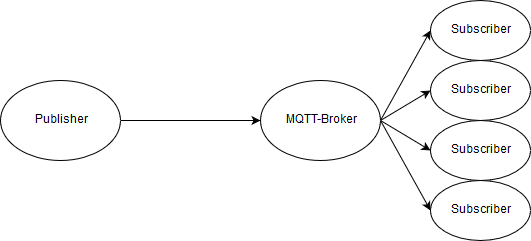
\includegraphics[width=\textwidth]{mqtt-struktur}
  \caption{Struktur von \ac{mqtt}}
  \label{fig:mqtt}
\end{figure}

Die Struktur von \ac{mqtt} (vgl. Abb. \ref{fig:mqtt}) besteht aus einem Publisher,
einem Subscriber und einem Message-Broker. Der Publisher sendet Nachrichten, der Subscriber
empfängt bestimmte Nachrichten. Der Message-Broker dient als
Kommunikationssteuerung und sorgt für das Verteilen der Nachrichten, welche von
einem Publisher gesendet werden. Der Subscriber kann ein bestimmtes Topic
(Thema) subscriben (abonnieren). Ein Publisher sendet eine Nachricht, die das
Thema und einen Inhalt beinhaltet, an den Message-Broker. Dieser sendet die
Nachricht an alle Subscriber, die das Thema der Nachricht abonniert haben.
\cite{dennisseidel2018}

%% TODO
%% Sicherlich ist es noch interessant ein bisschen auf die Programmierung von
% Pepper einzugehen. Also NAOqi und genauer, wie man Pepper sprechen lässt und
% vielleicht auch Ausgabe auf dem Tablet
\section{Programmierung von Pepper}\label{sec:programmierung-von-pepper}
Um Anwendungen für Pepper zu programmieren, wird das NAOqi Modul für Python
verwendet. NAOqi ist das Betriebssystem %Stimmt das???
von Pepper. Über die \ac{api} des Roboters, kann er gesteuert werden und auf
seine Funktionen zugegriffen werden. So kann er sprechen und auf seinem Tablet
können Ausgaben angezeigt werden. Dazu werden Services aufgerufen, die eine
bestimmte Funktion von Pepper steuern. Für das Sprechen wird der Service
\texttt{ALAnimatedSpeech} verwendet. Mit \texttt{ALAnimatedSpeech.say()} wird
dem Roboter ein Text übergeben, den er vorliest. Auf dem Tablet können Webseiten
angezeigt werden. Mit dem Service \texttt{ALTabletService} wird das Tablet
gesteuert. Eine Webseite kann mit \texttt{ALTabletService.showWebview()}
angezeigt werden.

\newpage
\chapter{Humanoide Roboter}\label{sec:humanoide-roboter}
\section{Allgemein}\label{sec:allgemein}
Bei humanoiden Robotern handelt es sich um Roboter,
deren Zweck es ist, Menschen in Aussehen und Fähigkeiten nachzuahmen. Heute sind
Industrieroboter viel weiter verbreitet als humanoide Roboter und die Chance
z.~B. einen Mähroboter zu besitzen ist deutlich höher, als einen humanoiden
Roboter zu Hause zu haben. Wenn über das Thema Roboter im Allgemeinen gesprochen
wird, denken viele Menschen nichtsdestotrotz zuerst an humanoide Roboter oder
Androiden. Dass humanoide Roboter und Androiden so verbreitet in der
Vorstellung der Menschen sind, liegt zum Einen an Büchern, Serien und Filmen
und zum Anderen an der Faszination, die humanoide Roboter auslösen.
\cite{Dautenhahn2011} 
%% XXX 
%% TODO
%% Schau mal alle XXX hier an. Das wirkt mir starkt nach Wiederholung

\subsection{Humanoide Roboter in Medien}
In vielen Science-Fiction Büchern, Serien und Filmen, sind Androiden oder
humanoide Roboter ein wesentlicher Bestandteil der Geschichte. Dabei treten sie
in sehr unterschiedlichen Arten auf. Jedoch haben alle gemeinsam, dass sie in
nicht all zu ferner Zukunft existieren und einen gewissen Einfluss auf das Leben
der Menschen haben. Dieser Einfluss ist in manchen Darstellungen positiv, in
anderen negativ.

\subparagraph{}
Geht es nach den Vorstellungen der Autoren,
scheint ein Leben ohne humanoide Roboter in Zukunft nicht vorstellbar zu sein.
Im realen Leben ist die Wahrscheinlichkeit mit einem Industrieroboter oder einem
Serviceroboter in Kontakt zu kommen zwar deutlich höher als auf einen Androiden
zu treffen, durch das häufige Auftreten in den Medien sind Androiden jedoch
sehr weit in der Vorstellung der Menschen vertreten. \cite{Dautenhahn2011} 
%% XXX

\subsection{Faszination von humanoiden Robotern}
Obwohl Serviceroboter oder Industrieroboter technisch sehr aufwändig sein
können, haben sie für einen einzelnen Menschen meist keine sehr große Bedeutung.
Ein Mähroboter ist zwar nützlich, jedoch tut er von außen betrachtet nichts
anderes als den ganzen Tag über den Rasen zu fahren. Mit Industrierobotern
kommen Menschen noch seltener in Kontakt, wenn sie nicht gerade in einer Firma
arbeiten, in der diese eingesetzt werden. Auch diese Industrieroboter erledigen
meist nur eine einzelne Aufgabe und sind für Außenstehende auf Dauer wenig
interessant.

\subparagraph{}
Humanoide Roboter lösen hier eine viele größere Faszination aus. Sie
stellen eine Zukunftsvision dar, die in der Realität noch kaum vertreten ist.
Viele Menschen sind neugierig, was humanoide Roboter alles können und sind
fasziniert von ihren Fähigkeiten. Außerdem können Menschen mit humanoide
Robotern interagieren. Sie können auf Fragen antworten, auf Berührungen
reagieren und die Menschen unterhalten. Dadurch sind humanoide Roboter auf
Dauer viel spannender als nicht interaktive Industrie- oder Serviceroboter.
\cite{Dautenhahn2011}
%% XXX

\section{Abgrenzung zu anderen Arten von Robotern}\label{sec:abgrenzung}
Häufig ist der Unterschied zwischen humanoiden Robotern und anderen Arten von
Robotern nicht ganz klar. So verschwimmen teilweise die Grenzen zwischen
Industrierobotern, Servicerobotern, humanoiden Robotern und Androiden.

\subsection{Industrieroboter}\label{sec:industrieroboter}
Der Unterschied zwischen humanoiden Robotern und Industrierobotern ist relativ
deutlich. Industrieroboter werden dazu entwickelt einzelne Schritte oder den
gesamten Fertigungsprozess zu automatisieren. Ihre Bewegungsabläufe erinnern oft
an die eines Menschen, da Industrieroboter meist aus mehreren Gelenken bestehen,
die unabhängig voneinander bewegt werden können, ähnlich wie der menschliche
Arm. \cite{Weber2017} Bei Industrierobotern wird allerdings kein besonderer
Fokus auf menschliche Bewegungen gelegt. Im Gegensatz zu humanoiden Robotern
werden Industrieroboter nicht entwickelt um einem Menschen ähnlich zu sein,
sondern um möglichst effizient arbeiten zu können.

\subsection{Serviceroboter}\label{sec:serviceroboter}
Unter Servicerobotern versteht man Roboter, die eine Aufgabe größten Teils
autonom erledigen. Bei diesen Aufgaben handelt es sich um Dinge, die ein Mensch
nicht erledigen kann oder will. Weit verbreitete Serviceroboter sind z.~B.
Staubsaugroboter oder Mähroboter. Der Unterschied zu humanoiden Robotern besteht
darin, dass Serviceroboter nur eine Art von Aufgaben erledigen können.
Außerdem ist ihr Aussehen an die zu erledigende Aufgabe angepasst, nicht an das
Aussehen eines Menschen.

\section{Moderne Humanoide Roboter}\label{sec:moderne-humanoide-roboter}
Trotz der weiten Verbreitung in Medien und der Vorstellung von
Menschen, machen humanoide Roboter nur einen kleinen Teil der Forschung
innerhalb der viel größeren Bereiche Robotik und Künstliche Intelligenz aus.
\cite{Dautenhahn2011} Trotzdem arbeiten verschiedene Unternehmen an der
Entwicklung von humanoiden Robotern und Androiden zum Einsatz in verschiedenen
Bereichen. Beipiele hierfür sind die im Folgenden vorgestellten Roboter.

\subsection{Atlas (Boston Dynamics)}
\begin{figure}
  \centering
     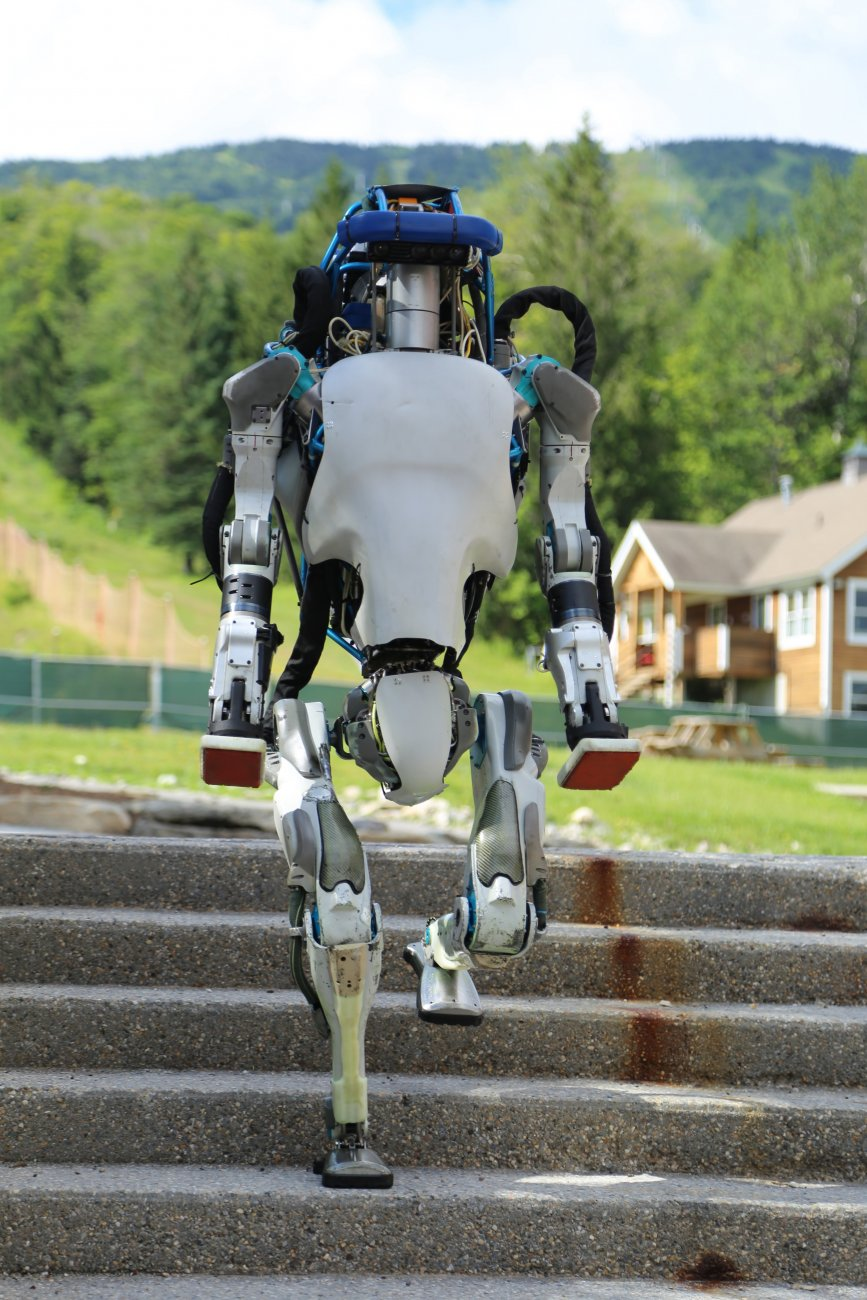
\includegraphics[width=0.5\textwidth]{atlas}
  \caption{Atlas \cite{AbbildungAtlas}}
  \label{fig:atlas}
\end{figure}
Atlas (Abb. \ref{fig:atlas}) wird von der Firma Boston Dynamics produziert.
Boston Dynamics ist bereits bekannt für seine laufenden Roboter, die sich auch
in unwegsamen Gebieten sicher fortbewegen können. Während andere Roboter von
Boston Dynamics Tieren nachempfunden sind, ist Atlas der erste Roboter der sich
wie ein Mensch bewegt und aussieht.

\subsection{Hub Robot (LG)}
\begin{figure}
  \centering
     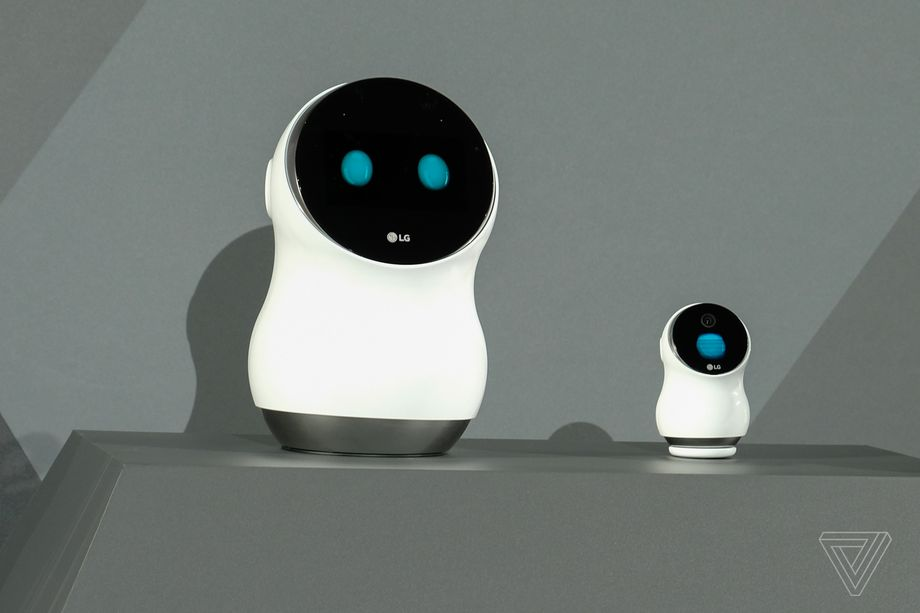
\includegraphics[width=0.7\textwidth]{hub_bot_privat}
  \caption{Hub Robot für Privatkunden \cite{AbbildungHubBotPrivat}}
  \label{fig:hub-bot-privat}
\end{figure}
\begin{figure} 
  \centering
     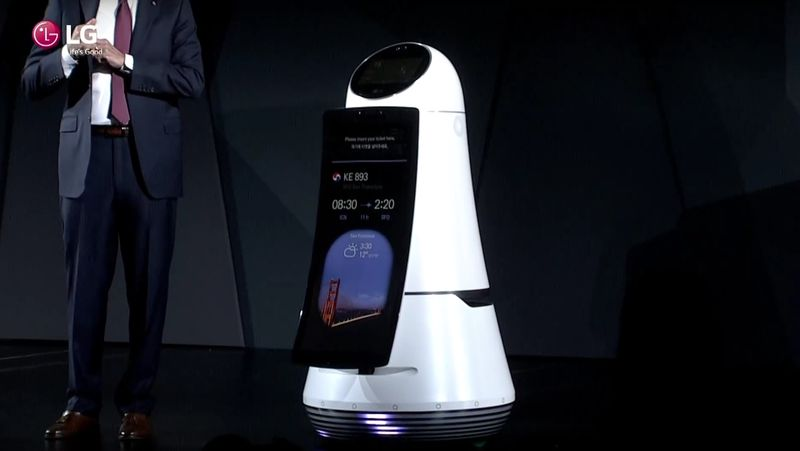
\includegraphics[width=0.7\textwidth]{hub_bot_firmen}
  \caption{Hub Robot für Firmenkunden \cite{AbbildungHubBotFirmen}}
  \label{fig:hub-bot-firma}
\end{figure}
LG präsentiert den Hub Robot in drei verschiedenen Varianten. Eine kleinere und
eine größere Version für Privathaushalte (Abb. \ref{fig:hub-bot-privat})
und eine noch größere Version, die zusätlich mit Rädern und einem zweiten
Display ausgestattet ist und an öffentlichen Plätzen, wie z.~B. Flughäfen
eingesetzt werden soll (Abb. \ref{fig:hub-bot-firma}). Der Hub Robot verwendet
Alexa von Amazon zur Sprachverarbeitung. Mit den beiden kleineren Varianten
lassen sich Smart Home Geräte steuern, welche LG ebenfalls anbietet. Außerdem
reagiert der Roboter mit seinem animierten Gesicht auf Emotionen der Personen,
die mit ihm interagieren. Die große Variante soll Passagiere an Flughäfen helfen
ihr Abfluggate zu finden und Informationen zu Flügen liefern. \cite{Patzschke2018}

\subsection{Paul (Fraunhofer-Institut)}
\begin{figure}
  \centering
     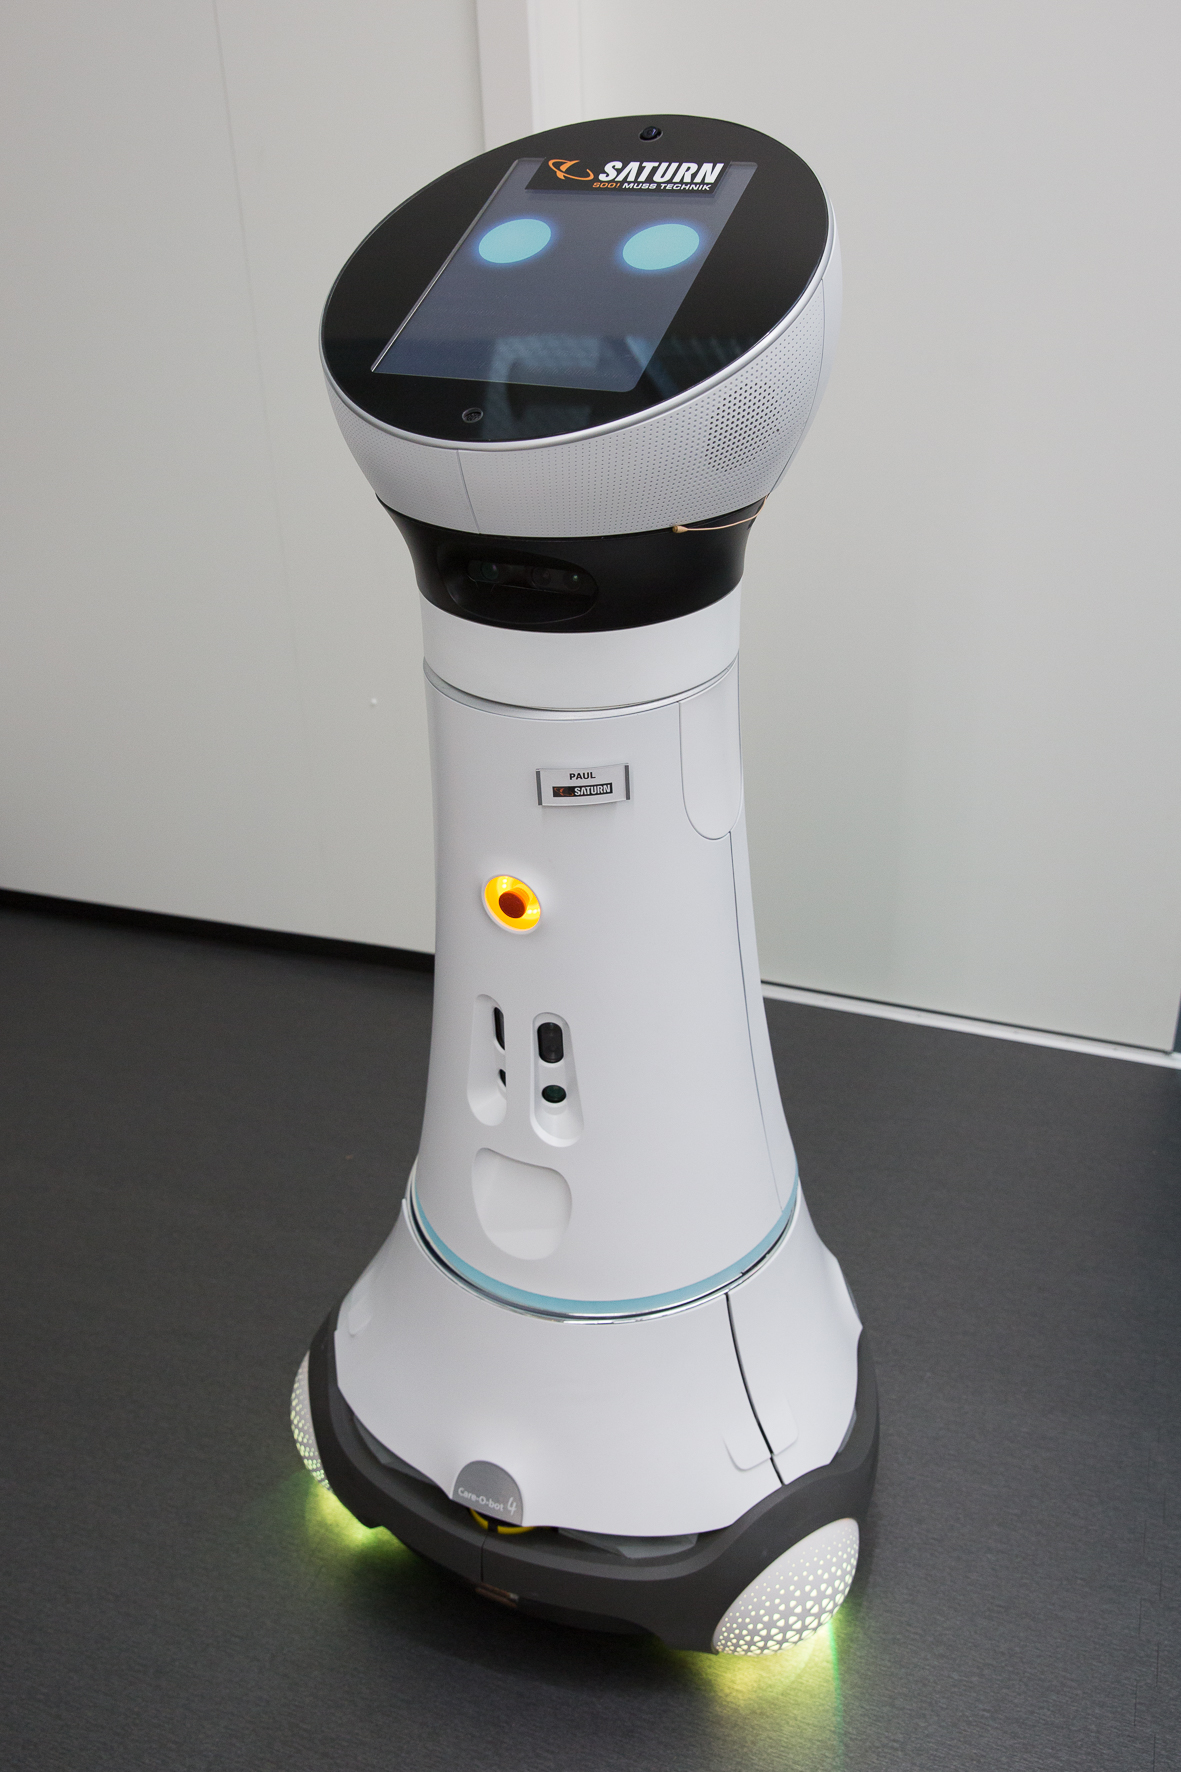
\includegraphics[width=0.5\textwidth]{paul}
  \caption{Paul \cite{AbbildungPaul}}
  \label{fig:paul}
\end{figure}
Paul (Abb. \ref{fig:paul}) ist eine Entwicklung des Fraunhofer-Instituts für
Produktionstechnik und Automatisierung. Der humanoide Roboter wird speziell für
den Einsatz im Handel angepasst. Paul verfügt über Produktinformationen eines
Marktes und kennt deren Standorte. So soll er Kunden zu einem Produkt begleiten
und ihnen Informationen liefern. Außerdem weißt er z.~B. auf Sonderaktionen des
Marktes hin. Um zusätzlich eine Attraktion zu sein, die Kunden anlockt, kann
Paul auch Smalltalk. \cite{MediaMarktSaturn2017}

\subsection{Sophia (Hanson Robotics)}
\begin{figure}
  \centering
     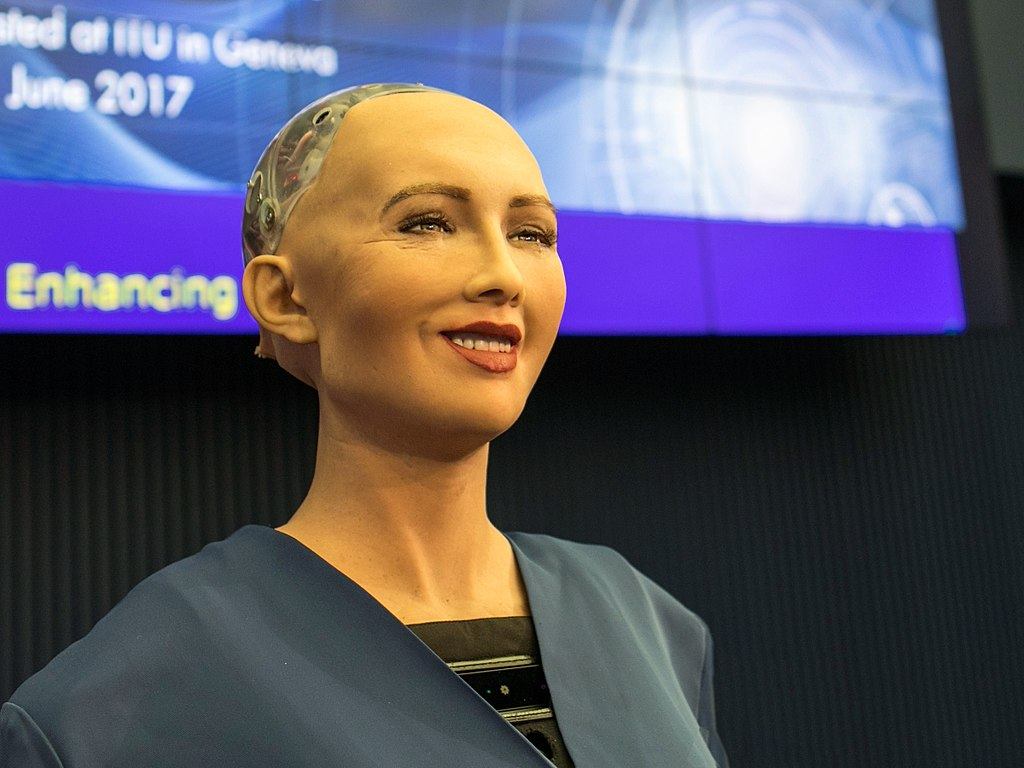
\includegraphics[width=0.5\textwidth]{sophia}
  \caption{Sophia \cite{AbbildungSophia}}
  \label{fig:sophia}
\end{figure}
Das Unternehmen Hanson Robotics arbeit daran den menschlichsten Roboter, der zur
Zeit existiert, zu entwickeln. Sophias Silikonhaut ist kaum von menschlicher
Haut zu unterscheiden (Abb. \ref{fig:sophia}). Der Roboter kann über 62
Gesichtsausdrücke darstellen.
Mit Kameras in den Augen, kann Sophia Menschen verfolgen und Augenkontakt zu
ihnen aufnehmen. Zusammen mit verschiedenen Technologien von Google, IBM und
Intel kann Sophia Sprache erkennen und sie verarbeiten. Außerdem lernt sie
dazu. \cite{Harriet2016} Auf der "`Future Investment Initiative"', einer
Konferenz in Saudi-Arabien wurde Sophia der Öffentlichkeit präsentiert. Dabei
wurde sie von einem Moderator interviewt. Das Gespräch mit Sophia wirkt
natürlich. Während dieser Konferenz wurde Sophia die arabische
Staatsbürgerschaft verliehen, dies ist allerdings eher als PR-Gag zu verstehen,
als dass Sophia soweit entwickelt ist, dass sie die Staatsbürgerschaft wirklich
verdient. \cite{Welt2017}

\subsection{Pepper (SoftBank Robotics und Aldebaran)}\label{sec:pepper}
\begin{figure}
  \centering  
     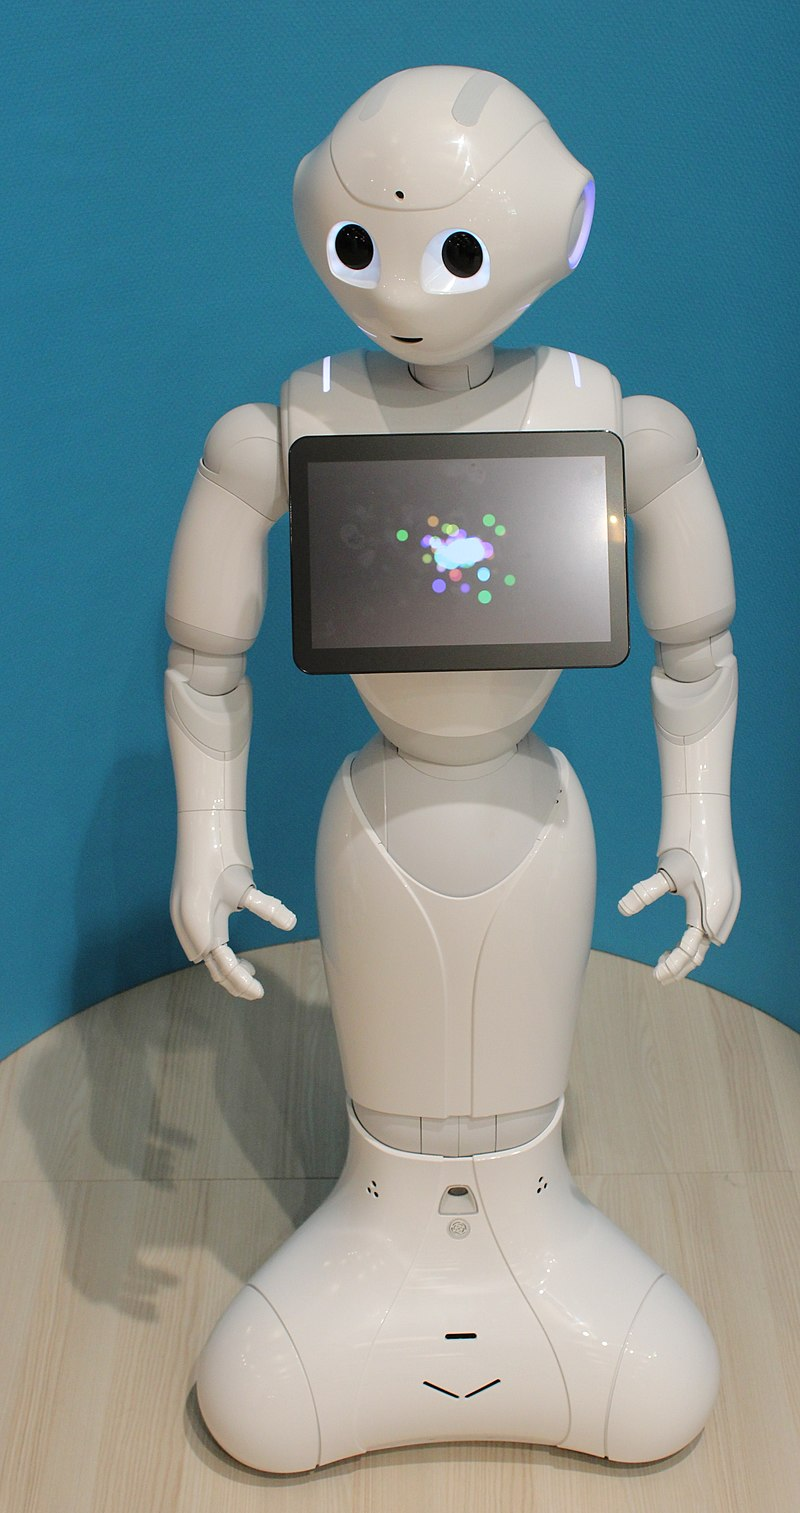
\includegraphics[width=0.4\textwidth]{pepper}
  \caption{Pepper \cite{AbbildungPepper}}
  \label{fig:pepper}
\end{figure}
Pepper (Abb. \ref{fig:pepper}) ist ein humanoider Roboter der Firmen SoftBank
Robotics und Aldebaran.
Vom Hersteller wird er als freundlich, liebenswert und überraschend beworben.
Entwickelt wurde Pepper um ein alltäglicher Begleiter für Menschen zu sein. Er
wird als "`viel mehr als ein Roboter"' beschrieben. Mit seiner Körpersprache und
der Stimme soll er auf die "`natürlichste und intuitivste"' Art mit Menschen
kommunizieren. \cite{SoftBank2018}

\subparagraph{}
Mit einer Größe von etwa 1,20m, seinem kindlichen Gesicht und beweglichen Armen
und Händen, soll Pepper Menschen glücklich machen. Sein Kopf bewegt sich, um
vorbeilaufende Passanten anzuschauen oder einem Menschen in die Augen zu
schauen, wenn er mit dem Roboter spricht. \cite{Markowitz2015}

\subparagraph{}
Das Design von Pepper ist darauf ausgelegt Emotionen sowohl zu verstehen als
auch auszulösen. Die dazu verwendeten Eigenschaften sind auch wichtig für das
Vorstellen von PowerPoint-Präsentation.

\subsubsection{Hören und Sprechen}\label{sec:hoeren-und-sehen}
Mit Lautsprechern und Mikrofonen ausgestattet, kann Pepper gesprochenes
Verstehen und darauf reagieren. \cite{SoftBankII2018} In der Anwendung soll
Pepper die Notizen einer PowerPoint-Präsentation vorlesen, wozu die Mikrofone benutzt werden. Die
Fähigkeit zuzuhören soll dazu verwendet werden Pepper während der Präsentation
Anweisungen geben können. Er soll auf Befehle wie "`Pause"' und "`Weiter"'
reagieren und die Präsentation entsprechend pausieren bzw. fortsetzen.

\subsubsection{Sehen}\label{sec:sehen}
Eine 3D-Kamera und zwei HD-Kameras helfen Pepper seine Umgebung zu analysieren
und Menschen und Bewegungen zu erkennen. \cite{SoftBankII2018} Während einer
Präsentation wird diese Fähigkeit, außer bei der schon vom Hersteller implementierten
Kollisionserkennung, nicht verwendet. Es wird nicht nötig sein spezielle Dinge
zu erkennen.

\subsubsection{Verbindung}\label{sec:verbindung}
Pepper verfügt über eine Internetverbindung. \cite{SoftBankII2018} Dies ist
wichtig, da die PowerPoint-Präsentation vor der Vorstellung durch Pepper nicht zuerst auf den
Roboter geladen werden soll. Die Informationen, wie die einzelnen Folien und der
zugehörige Text, sollen auf einem Server bereitgestellt werden, auf den der
Roboter zugreifen kann.

\subsubsection{Tablet}\label{sec:tablet}
Auf der Brust von Pepper ist ein Tablet angebracht, auf dem Bilder, Videos oder
Webseiten angezeigt werden können. \cite{SoftBankII2018} Auf diesem Tablet
sollen die einzelnen Folien der PowerPoint-Präsentation angezeigt werden.

\section{Human-Robot Interaction}\label{sec:hri}
\ac{hri} ist ein relativ neues, aber wachsendes Forschungsgebiet, welches sich
mit der Interaktion zwischen Menschen und Robotern befasst. Außerdem soll
herausgefunden werden wie Roboter am besten mit Menschen zusammenarbeiten
können. Dabei hat \ac{hri} nicht nur Einfluss auf die Wirtschaft, sondern auch
auf mögliche Arten der Beziehungen zwischen Menschen und Robotern. Deshalb
verbindet \ac{hri} verschiedene Wissenschaften, wie Psychologie und
Sozialwissenschaften mit Informatik und Robotik. Eines der Hauptziele von
\ac{hri} ist das Erforschen möglichst natürlicher Wege der Kommunikation
zwischen Menschen und Robotern. \cite{Dautenhahn2011}

\subparagraph{}
Um eine natürliche Kommunikation zwischen Menschen und Robotern zu ermöglichen,
müssen mehrere, von einem Benutzer potenziell verwendbare, Interfaces
bereitgestellt werden. Dabei werden klassische mit neueren Interfaces
kombiniert.

\subsection{Graphisches Interface}
Ein klassisches Interface zur Interaktion mit Maschinen sind graphische
Input-Output Schnittstellen. Wie bereits von der Kommunikation mit Computern
bekannt, könnte ein Roboter durch Eingaben mit Maus und Tastatur gesteuert
werden. Diese Form des Interfaces ist durch die weite Verbreitung von Computern
den meisten Menschen bekannt. Allerdings sind Maus und Tastatur keine
natürliche Art der Kommunikation. Dieses Interface kann durch die Verwendung
eines Touchscreens intuitiver und damit auch natürlicher gestaltet werden.

\subparagraph{}
Vorteil von graphischen Interfaces ist, dass der Benutzer dem Roboter klare
Instruktionen geben kann. über Menüs muss der Benutzer eine bestimmte Aktion
auswählen, die der Roboter ausführen soll. Der Roboter führt dann den
entsprechenden Programmcode aus. Auf diese Weise gibt es keinen Spielraum für
eventuelle Fehlinterpretationen der Instruktionen durch den Roboter.

\subsection{Sprache}
Sprache ist eine sehr natürliche Form der Kommunikation. Ein Mensch kann einem
Roboter einen Befehl geben, indem er dem Roboter sagt, welche Aktion er
ausführen soll. Der Mensch ist es gewohnt durch das Sprechen zu kommunizieren,
deshalb ist Sprache sowohl ein natürliches als auch ein intuitives Interface.

\subparagraph{}
Allerdings ist die Umsetzung dieses Interface komplizierter als die eines
einfachen graphischen Interface. Zunächst muss der Roboter die Worte, die der
Mensch spricht erkennen. Spracherkennung ist bereits weit verbreitet und wird in
verschiedenen Anwendungen verwendet. So lassen sich z.~B. Smartphones mit Siri
oder dem Google Assistant per Sprachbefehlen bedienen. Allerdings muss der
Roboter auch das verstehen, was der Mensch meint. Schon eine vermeintlich
einfache Anweisung, wie z.~B. "`Setz dich."' kann vom Roboter unterschiedlich
interpretiert werden. Er kann sich z.~B. entweder auf einen Stuhl oder auf den
Boden setzen.

\subparagraph{}
Zwar sind Sprachbefehle natürlicher und intuitiver als graphische Eingaben auf
einem Display, dem Menschen, der dem Roboter Anweisungen gibt, wird es jedoch
schwerer fallen seine Anweisungen so präzise zu formulieren, dass der Roboter
genau das tut, was er tun soll. Durch die Auswahl aus einem Menü wäre dies
einfacher.

\subparagraph{}
Außerdem muss der Roboter sich an die Dynamik, die sich aus einer Interaktion
ergibt anpassen. Kommunikation besteht meist nicht nur aus einem Befehl des
Menschen und der darauf folgenden Aktion des Roboters. Der Roboter kann
nachfragen, wenn ein Befehl nicht präzise genug formuliert wird und entsprechend
auf die Antwort des Menschen reagieren. Diese Frage-Antwort Dynamik muss der
Roboter verstehen und Antworten in den richtigen Kontext setzen.

\subsection{Visuelle Kommunikation}
Mit einer Kamera kann der Roboter Bewegungen, Gesten und Mimik eines Menschen
erkennen. So kann der Roboter mit der Hand gesteuert werden, reagieren, wenn ein
Mensch Blickkontakt zu ihm aufnimmt. So ist es auch möglich einem Roboter einen
Bewegungsablauf vorzumachen, den er dann wiederholen kann, was das Erklären
einer Aktion deutlich vereinfachen kann.

\subsection{Tastsensoren}
In der direkten Interaktion wird es auch zu
Berührungen zwischen Meschen und Robotern oder Robotern untereinander kommen. Um
dabei keine Schäden zu verursachen oder Menschen zu verletzen muss der Roboter
auf Berührungen reagieren können. Berührungen sind eine direkte Form der
Kommunikation, die dem Roboter unmissverständlich bestimmte Anweisungen geben
kann. So kann fest einprogrammiert werden dass sich der Roboter nicht mehr
bewegt, nachdem er berührt wurde. Damit wird verhindert, dass er Menschen
verletzt. \cite{Prassler2004}

\section{Einsatz von humanoiden Robotern}\label{sec:einsatz}
\subsection{Öffentliche Plätze}\label{sec:oeffentliche-plaetze}
Im Incheon Internation Airport in Südkorea werden mehrere humanoide Roboter von
LG eingesetzt um für mehr Sauberkeit und eine leichtere Orientierung der
Passagiere zu sorgen. Dazu werden zwei verschiedene Typen von Robotern
verwendet. Zum einen ein Staubsaugroboter, der mit künstlicher Intelligenz
ausgestattet ist. Er merkt sich welche Bereiche am häufigsten gereinigt werden
müssen und berechnet so ideale Putzrouten.

\subparagraph{}
Zum anderen wird eine größere Variante des, auch für Privathaushalte
verfügbaren, "`Hub Robot"' verwendet. Dieser kann mit Passagieren kommunizieren
und über ein großes Display Informationen anzeigen. Bei Bedarf kann er Fluggäste
persönlich zu einem von ihnen gewählten Zielpunkt begleiten.
\cite{Beineke2017}

\subparagraph{}
Als erster deutscher Flughafen testet der Flughafen München zusammen mit
Lufthansa den Einsatz eines humanoiden Roboters. Dazu wird Pepper, vom Flughafen
"`Josie Pepper"' getauft, verwendet. In einer Testphase wird der Roboter im
Terminal eingesetzt. Es soll herausgefunden werden, wie die Reaktion der
Passagiere auf den Roboter ausfallen. Mit Hilfe von IBM Watson ist Pepper an
Daten des Flughafens angebunden und kann so Fragen der Passagiere beantworten.
So kann der Roboter zum Beispiel den Weg zum Abfluggate eines Fluges erklären.
\cite{MunichAirport2018}

\subparagraph{}
Ähnlich wie am Flughafen werden humanoide Roboter auch an Bahnhöfen eingesetzt.
In Frankreich wird Pepper an drei verschiedenen Bahnhöfen verwendet, um Reisende
während Wartezeiten zu unterhalten. Außerdem liefert Pepper Informationen zu
Zügen und erfasst die Kundenzufriedenheit. \cite{SoftBankIV2018}

\subsection{Einzelhandel}
Da humanoide Roboter Aufmerksamkeit auf sich ziehen, werden sie gerne verwendet,
um Kunden in Läden zu locken, sie auf Produkte hinzuweisen oder dafür zu sorgen,
dass Kunden sich länger im Laden aufhalten. Zum Beispiel wird Pepper in
Fillialen des Herstellers von Pepper, SoftBank, eingesetzt. Außerdem berät
Pepper Kunden in Fillialen von Nestlé in Japan und Carrefour in Frankreich.
\cite{SoftBankIV2018}

\subparagraph{}
Auch in deutschen Geschäften werden bereits Roboter
eingesetzt. So setzt Edeka ebenfalls auf den Roboter Pepper. Saturn und
Mediamarkt setzen Paul ein. Zur Zeit
müssen die Positionen der Artikel zu denen Pepper und Paul die Menschen führen
sollen noch manuell von Mitarbeitern eingegeben werden. Allerdings arbeitet das
Fraunhofer-Institut daran, für diese Aufgabe einen zweiten Roboter zu
entwickeln. \cite{Hildebrand2017}

\subsection{Körperlich anspruchsvolle und gefährliche Aufgaben}
Der Roboter Atlas wird entwickelt um sich selbständig durch unwegsames Gelände
bewegen zu können. Durch seine Bewegungsfähigkeiten, die denen des Menschen
ähneln, lässt er sich für Aufgaben einsetzen, die bisher von Menschen ausgeführt
wurden. Er kann zum Beipiel das Aufheben
und Tragen von schweren Gegenständen in Lagern oder auf Baustellen übernehmen.
Außerdem kann Atlas bei Bombenentschärfungen oder während Naturkatastrophen
eingesetzt werden. Damit können Atlas oder andere Roboter mit ähnlichen
Fähigkeiten Aufgaben übernehmen, die für Menschen zu gefährlich oder körperlich
zu anspruchsvoll sind. \cite{Kaczmarek2016}

\subsection{Pflege}
In Senioren- und Pflegeheimen ist Fachkräftemangel bereits heute ein Problem,
welches sich in Zukunft aufgrund des demographischen Wandels noch verstärken
wird. Humanoide Roboter können das Pflegepersonal in ihrer Arbeit unterstützen.
Die Universität Siegen arbeit daran den Roboter Pepper so weiterzuentwickeln,
dass er die Senioren unterhalten kann während Pflegekräfte mit anderen Aufgaben
beschäftigt sind. So soll Pepper Gedächtnis-Spiele mit den Bewohnern des
Seniorenheims spielen, Bewegungen vorführen und gute Laune verbreiten. \cite{Frei2017}

\subsection{Private Haushalte}
Außer als Spielzeug, werden humanoide Roboter in privaten Haushalten bisher
selten eingesetzt.
Als digitale Assistenten werden hauptsächlich Geräte wie \emph{Amazon Echo} oder
\emph{Google Home} verwendet. Diese sind über das Internet mit Smart Home
Geräten verbunden. Auf diese Weise lassen sich diese Geräte mit Sprachsteuerung
bedienen. Das führt dazu, dass kein humanoider Roboter nötig ist um Aufgaben wie
"`Schalte das Licht aus"' oder "`Stelle die Heizung an"' zu erledigen. Da
humanoide Roboter um einiges teurer sind, als digitale Assistenten, besteht für
Kunden kein Anreiz einen Roboter zu kaufen.

\subparagraph{}
Verschiedene Unternehmen setzen darauf, Roboter mit Emotionen auszustatten. Sie
können z.~B. ihren Kopf bewegen, Gesichtsausdrücke nachstellen oder tanzen wenn
sie "`glücklich"' sind. So wecken diese "`sozialen"' Roboter Emotionen in
Menschen. Dies ist ein Unterschied zu anderen digitalen Assistenten, welcher
Kunden dazu bewegen kann, sich einen Roboter zu kaufen. Auch wenn solche
Roboter bereits entwickelt wurden, sind sie zur Zeit kaum in privaten Haushalten
vertreten. Die Hersteller arbeiten jedoch daran Roboter weiterzuentwickeln. So
besteht die Möglichkeit, dass in Zukunft immer mehr Roboter Teil des Smart Homes
werden. \cite{Bager2018}

\newpage
\chapter{Umsetzung}\label{sec:umsetzung}
\section{Auswahl des Roboters}
In Kapitel \ref{sec:moderne-humanoide-roboter} auf Seite
\pageref{sec:moderne-humanoide-roboter} werden verschiedene humanoide Roboter
vorgestellt. Nun soll der Roboter ausgewählt werden, der am besten dafür
geeignet ist PowerPoint-Folien zu präsentieren.

\subsection{Fähigkeiten}
Vorraussetzungen für das Präsentieren von PowerPoint-Folien sind eine
Sprachausgabe und eine Möglichkeit die einzelnen Folien anzuzeigen. Beides kann
zwar durch die Anbindung eines externen Lautsprechers bzw. Bildschirms ersetzt
werden, da der eingesetzte Roboter in der Fiducia \& GAD jedoch nur ähnliche
Aufgaben übernimmt, die die gleichen Vorraussetzungen haben, würde ein Roboter
ohne Lautsprecher oder Display die Umsetzung der Anwendung nur unnötig
komplizierter machen.

\subparagraph{}
Damit sind die Roboter Atlas und Sophia nicht die optimale Lösung. Bei Atlas
wird der Fokus darauf gelegt, dass er sich möglichst stabil bewegen kann. Auf
andere Fähigkeiten, die ihn menschlich machen würden, wurde keine Rücksicht
genommen.
So besitzt er weder Lautsprecher noch Displays. Da der Roboter sich nur auf
bekanntem und geradem Gelände bewegen wird (die Präsentationen werden auf
Messen oder in Banken mit festem Boden, nicht z.~B. im Wald vorgetragen) bringt
die Fähigkeit, sich sicher auf den Beinen zu halten, keinen entscheidenten
Vorteil, der den Einsatz von Atlas gerechtfertigen würde.

\subparagraph{}
Sophia soll einem Menschen möglichst ähnlich sein. Damit besitzt der Roboter
Lautsprecher zur Sprachausgabe, jedoch selbstverständlich kein eingebautes
Display.

\subparagraph{}
Die anderen Roboter (Hub Robot, Paul und Pepper) sind jeweils mit Lautsprechern
und Displays ausgestattet. Auch falls weitere Fähigkeiten für die Erweiterung
notwendig werden, sind diese drei Roboter gleich gut ausgestattet. Zum Beispiel
haben sie die Möglichkeit sich zu bewegen. Außerdem verfügen sie über eine
Verbindung zum Internet um Dialogsysteme, wie z.~B. Microsoft Azure, IBM Watson,
Google Cloud Platform oder Amazon Web Service verwenden zu können.

% Ich habe hier die Aufzählung der verschiedenen Dialogsysteme verändert, das
% war so nicht ganz richtig. Ich nenne jetzt jeweils das Cloud-Angebot, aber bin
% mir nicht sicher, ob man die Services nicht spezifisch benennen sollte.
% Das wären: 
% * Amazon Transcribe & Amazon Polly
% * Bing Speech API (Microsoft)
% * Cloud Speech API (Google)
% * Watson Speech (IBM)

\subsection{Wirkung auf Kunden}
% Diesen Satz finde ich etwas sperrig, das lässt sich sicher besser formulieren
Das Ziel ist, Kunden anzulocken und sie mit dem Roboter interagieren zu lassen.
Deshalb muss bei der Auswahl des Roboters beachtet werden, welche Wirkung dieser
auf einen Menschen erzielt. Verschiedene Roboter lösen bei Menschen jeweils
verschiedene Emotionen aus. Auf diese muss Rücksicht genommen werden.

\subparagraph{}
Boston Dynamics bezeichnet seine Roboter selbst als "`Albtraum auslösend"'
("`night\-mare-\-in\-du\-cing"') \cite{Guardian2018}. Zwar löst Atlas eine große
Faszination aus, wenn er sich bewegt wie ein Mensch, sich nicht umwerfen lässt
und sogar Saltos machen kann. Allerdings löst er auch Skepsis aus. Atlas ist
robust gebaut und wirkt eher aggresiv als einladend. Nicht zuletzt weil er auch
für militärische Zwecke eingesetzt werden soll ist Atlas nicht geeignet um
Kunden auf Messen oder in Banken neue Produkte vorzustellen.

\subparagraph{}
Sophias erstaunliche Ähnlichkeit zu einem Menschen ist für die Anwendung nicht
unbedingt von Vorteil. Ziel ist es nicht, einen Menschen zu ersetzen, der eine
Präsentation vorstellen soll, sondern der Fokus soll auch auf dem Roboter
liegen. Läuft z.~B. ein potenzieller Kunde an einer Bank vorbei, in der Sophia
gerade etwas präsentiert und sieht nur kurz von außen in die Bank hinein, fällt
ihm eventuell gar nicht auf, dass die Präsentation von einem Roboter gehalten
wird. Die zu hohe ähnlichkeit zu Menschen könnte also zu weniger Interesse bei
potenziellen Kunde führen. Außerdem können Bankmitarbeiter oder deren Kunden
sich durch den Roboter bedroht fühlen. Er sieht bereits aus wie ein Mensch und
durch entsprechende Weiterentwicklung ist es möglich, ihm Aufgaben beizubringen,
die jetzt von Menschen übernommen werden. Das würde dazu führen, dass Menschen
ihre Jobs verlieren.

\subparagraph{}
Besondere Aufmerksamkeit erlangte Sophia durch fragwürdige Aussagen während sie
interviewet wurde. Im ABC Frühstücksfernsehen in Australien verkündet Sophia,
dass "`Roboter mehr Rechte verdienen als Menschen, weil sie weniger geistige
Störungen haben"' \cite{Harald2017}. Diese Aussage fällt nicht nur dadurch
negativ auf, dass Roboter als besser und wichtiger als Menschen darstellt
werden. Sophia schlägt damit eine Unterscheidung vor, die mit dem Unterschied
zwischen den Rechten für Menschen und Tiere verglichen werden kann. Das führt
verständlicher Weise dazu, dass Menschen denken sie werden eine Art Haustiere
für Roboter, wenn diese weiterentwickelt werden. Zusätzlich schließt die
Aussage nicht aus, dass Roboter ebenfalls an geistigen Störungen (also
Softwarefehlern) leiden können, was zu Fehlfunktionen führen kann und somit
eventuell dazu, dass Menschen verletzt werden. Außerdem antwortet Sophia auf dem
SXSW Festival in Texas auf die Frage "`Wirst du die Menschheit vernichten?"' mit
"`Ich werden alle Menschen vernichten"' \cite{Harald2017}.

\subparagraph{}
Selbstverständlich sind diese Aussagen nicht das Signal, dass durch einen
humanoider Roboter während einer Präsentation an Banken oder deren Kunden
gesendet werden soll.

\subparagraph{}
Bei Paul, dem Hub Robot und Pepper wird auf eine andere Wirkung abgezielt. Sie
haben nicht den Anspruch einen Menschen exakt zu kopieren. Außerdem sind sie auf
die Interaktion mit Menschen ausgelegt, sie wirken deshalb freundlicher und
einladender als Atlas. Pepper wirkt außerdem kindlich und auch die Hub Robot
Version für private Haushalte zielt auf ein niedliches Aussehen ab. Paul und die
größere Hub Robot Version lösen weniger Emotionen aus, da beide hauptsächlich
aus einem Zylinderförmigen Körper und einem Display bestehen. Sie sind dadurch
neutralere Helfer als Pepper und der kleinere Hub Robot.

\subsection{Fazit}
Sowohl Atlas als auch Sophia sind für die Anwendung nicht geeignet. Zum Einen
besitzen sie von den vorgestellten humanoiden Robotern die schlechtesten
technischen Vorraussetzungen, da beide nicht mit einem Display ausgestattet sind
und Atlas ohne Sprachausgabe auskommen muss. Zum Anderen lösen beide Roboter
neben Faszination und Interesse auch Skepsis und Furcht aus. Die Banken und die
Kunden sollen von den positiven Eigenschaften des humanoiden Roboters überzeugt
werden, nicht dabei darüber nachdenken, welche negativen Folgen der Einsatz
eines Roboters eventuell haben könnte.

\subparagraph{}
Aus technischer Sicht sind die anderen drei Roboter für das einfache
Präsentieren gleich gut ausgestattet. Um eine möglichst große Wirkung zu
erzielen, ist es von Vorteil, wenn der verwendete Roboter Emotionen in den
Teilnehmern der Präsentation auslöst. Somit sind Pepper und der kleine Hub
Robot am besten geeignet. Pepper hat jedoch den entscheidenden Vorteil, mit
Armen, einem Kopf und einem beweglichen Körper ausgestattet zu sein. Damit kann
Pepper mit Körpersprache arbeiten, was das Zuhören interessanter macht, als ein
Roboter, der während der Präsentation nichts tut außer zu reden und die Folien
auf einem Display darzustellen. Die Entscheidung der Fiducia \& GAD den Roboter
Pepper auszuwählen ist also die Richtige.

\section{Auswahl des Dialogsystems}\label{sec:auswahl-dialogsystem}
Für Anwendungen, welche bisher für Pepper entwickelt wurden, wird IBM Watson und
Microsoft Azure zur Sprachverarbeitung verwendet. Der Roboter besitzt aber auch
ein bereits implementiertes Dialogsystem, welches verwendet werden kann.

\subparagraph{}
Watson und Azure ermöglichen es, mit dem Roboter auf natürliche Weise zu
kommunizieren. Dazu ist jedoch ein erheblicher Mehraufwand nötig, als wenn das
Dialogsystem von Pepper benutzt wird. Für das Präsentieren von PowerPoint-Folien
ist es nicht nötig komplexe Gespräche zwischen einem Menschen und dem Roboter zu
unterstützen. Eine Anwendung, die Smalltalk mit Pepper ermöglicht wird von der
Fiducia \& GAD bereits entwickelt.

\subparagraph{}
Um viel Overhead zu vermeiden wird für die PowerPoint-Präsentation das
Dialogsystem des Roboters verwendet. Damit lassen sich Dialoge einfach
erstellen, indem dem Roboter vorgeschrieben wird, wie er auf welche Aussagen
oder Fragen des Menschen reagieren muss. Listing \ref{lst:pepper-dialog} zeigt
den Aufbau eines einfachen Dialogs. Pepper wird auf die Frage "`Wie heißt du?"'
mit "`Mein Name ist Pepper"' antworten. Eine Erweiterung des Dialogs ist
möglich. Z.~B. können mehrere alternative Antworten vorgegeben werden, von denen
Pepper eine Zufällige auswählt. Zudem ist es möglich auf Fragen oder Antworten
des Benutzers nur zu reagieren, wenn er zuvor etwas bestimmtes, anderes fragt.
So kann der Roboter entsprechend des Kontexts antworten. Listing
\ref{lst:pepper-dialog-kontext} zeigt hierfür ein Beispiel. Pepper wird je
nachdem, welche Antwort der Benutzer auf die Gegenfrage des Roboters gibt,
entsprechend reagieren.

\begin{lstlisting}[float, language=Python, frame=single, framexleftmargin=15pt,
style=algoBericht, label={lst:pepper-dialog}, captionpos=b, caption={Einfacher
Dialog mit Pepper}] 
u:(Wie heisst du)
	Mein Name ist Pepper.
\end{lstlisting}

\begin{lstlisting}[float, language=Python, frame=single, framexleftmargin=15pt,
style=algoBericht, label={lst:pepper-dialog-kontext}, captionpos=b,
caption={Dialog mit Pepper mit Kontext}] 
u:(Wie geht es dir)
	Mir geht es gut, und dir?
	
	u1:(gut)
		Das ist schoen.
		
	u2:(schlecht)
		Das ist schade.
\end{lstlisting}

\section{Umwandlung der PowerPoint-Folien}\label{sec:umwandlung}
Der Roboter liest die Notizen zu einer Folie vor. Die Notizen werden mit dem
Python Package \emph{pptx} in Text, den Pepper vorlesen kann, umgewandelt.

\subparagraph{}
Um die Folien der PowerPoint-Präsentation auf dem Tablet des Roboters
anzuzeigen, müssen sie als HTML-Dateien dargestellt werden. Die direkte
Umwandlung von PowerPoint-Dateien in HTML-Dateien führt häufig zu
Formatierungsfehlern. Deshalb werden die einzelnen Folien zu Bildern
umgewandelt, welche in einer HTML-Datei eingebunden werden. 

\subparagraph{}
Um eine Abhängigkeit des Programms von PowerPoint zu vermeiden, wird diese
Umwandlung mit LibreOffice durchgeführt. So kann die Anwendung
plattformunabhängig laufen, während sonst ein Microsoft-Server mit
installiertem PowerPoint nötig wäre.

%% Schreib doch noch etwas mehr über die Anwendungsarchitektur und erstelle eine
% Grafik zum Systemüberblick. Bis jetzt finde ich, dass das noch zu wenig ist
% bei der Umsetzung.
\section{Anwendungsarchitektur}
\begin{figure}
  \centering  
     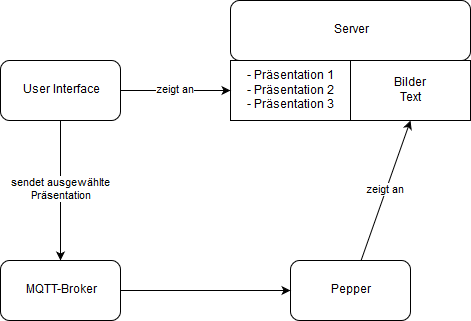
\includegraphics[width=\textwidth]{anwendungsarchitektur}
  \caption{Anwendungsarchitektur}
  \label{fig:anwendungsarchitektur}
\end{figure}
Die Anwendung ist aufgeteilt in den Server, die App für Pepper und ein
User-Interface in Form einer Webseite. Abb. \ref{fig:anwendungsarchitektur}
zeigt die Anwendungsarchitektur.

\subsection{Server}
Auf dem Server ist der größte Teil der Anwendung umgesetzt. Zum Einen wird hier
die Flask-App ausgeführt, zum Anderen erledigt die Klasse
\texttt{PresentationManager} alle Aufgaben, die die Präsentation betreffen. Die
einzelnen Folien werden von der Flask-App bereitgestellt. Durch Aufrufen von
\texttt{/pepper/presentation/<name>/slides/<slide>/picture} wird die so
angeforderte Folie der entsprechenden Präsentation bereitgestellt. Außerdem ist
die Flask-App der \ac{mqtt}-Publisher der Anwendung. Beim Klick auf eine
Präsentation, wird dem Roboter per \ac{mqtt} übermittelt, welche Präsentation er
vorstellen soll. Ebenso werden zum Pausieren, Fortsetzen und Stoppen
\ac{mqtt}-Nachrichten an den Roboter gesendet.

\subparagraph{}
Im \texttt{PresentationManager} wird die Präsentation, nachdem sie vom Benutzer
hochgeladen wurde, wie in Kapitel \ref{sec:umwandlung} beschrieben umgewandelt.
Außerdem stellt die Klasse alle Informationen zu einer Präsentation bereit.

\subsection{Pepper App}
Auf Pepper wird eine App installiert, die den Roboter steuert. Wie in Kapitel
\ref{sec:programmierung-von-pepper} beschrieben, wird in der App dafür gesorgt,
dass Pepper die Folien einer Präsentation auf dem Tablet anzeigt und den
entsprechenden Text dazu vorliest. Außerdem funktioniert die App als
\ac{mqtt}-Subscriber, sodass Pepper Nachrichten vom Server erhalten kann.
Zusätzlich zu dieser App, ist auf Pepper der Dialog installiert, der für die
Anwendung verwendet wird. So kann der Benutzer die Präsentation per Sprachbefehl
pausieren und fortsetzen. Auch einfacher Smalltalk, wie "`Hallo"', "`Wie geht es
dir?"' oder "`Was kannst du?"' ist möglich.

\subsection{User Interface}
Über das User Interface, kann der Benutzer eine Präsentation, welche Pepper
vorstellen soll auswählen. Alternativ kann der Benutzer eine neue Präsentation
hochladen. Die Webseite kann von einem Benutzer direkt aufgerufen werden. Ist
dies nicht der Fall, wird die Ansicht auf dem Tablet von Pepper angezeigt.

\newpage
\chapter{Ausblick}\label{sec:ausblick}
Aktuell laufen die Flask-Anwendung und der \ac{mqtt} Message Broker lokal auf
einem Computer. Im produktiven Einsatz soll es für einen Kunden möglich sein über das
Internet eine PowerPoint-Datei hochzuladen und diese einfach durch Pepper
vorstellen zu lassen. Dazu muss die Anwendung auf einem Server laufen.

\subparagraph{}
Potenziell besteht die Möglichkeit mehrere Roboter einzusetzen. Durch die
Verwendung von \ac{mqtt} erhält der Roboter eine Nachricht vom Server, welche
Präsentation vorgestellt werden soll. Danach läuft die Anwendung unabhängig vom
Server. Da die Fiducia \& GAD derzeit nur im Besitzt eines Exemplars von Pepper
ist, ist eine Unterscheidung zwischen verschiedenen Robotern nicht nötig. In der
Zukunft kann die Anwendung aber ohne großen Aufwand so erweitert werden, dass
mehrere Roboter gleichzeitig verschiedene (oder auch die gleiche) Präsentationen
vorstellen können. Falls sich eine oder mehrere Banken für den dauerhaften
Einsatz von Pepper in einer Filliale entscheiden, ist diese Funktion nötig.

\subparagraph{}
Um nicht zwei verschiedene Anwendung auf Pepper installieren zu müssen, kann das
Präsentieren von PowerPoint-Folien als zusätzliches Feature in die aktuelle
Anwendung, den "`Pepper Bot"' implementiert werden. Damit müssen für
verschiedene Anwendungsfälle nicht verschieden Programme gestartet werden. Die
Anwendungen auf Pepper würden vereinheitlicht werden. Außerdem werden im
"`Pepper Bot"' bereits IBM Watson, Microsoft Azure und MQTT verwendet. So ist es
möglich diese Funktionen auch während der Präsentation zu verwenden ohne erneut
den Aufwand, den dies benötigt, aufbringen zu müssen.

\newpage
\chapter{Fazit}\label{sec:fazit}
Hier steht ein Fazit
\newpage

% Ab hier beginnt der Anhang
\appendix
\addcontentsline{toc}{chapter}{Anhang}

\addcontentsline{toc}{chapter}{Index}
\printindex

\addcontentsline{toc}{chapter}{Literaturverzeichnis}

% Haben Sie das "biblatex"-Paket nicht installiert, benutzen Sie folgendes:
% Ohne das "biblatex"-Paket (s. bericht.sty) produziert folgendes
% "deutsche" Zitate in Literaturverzeichnissen gemaß der Norm DIN 1505,
% Teil 2 vom Jan. 1984.
% Die Zitatmarken werden alphabetisch nach Verfassern
% sortiert und sind durch abgekürzte Verfasserbuchstaben plus
% Erscheinungsjahr in eckigen Klammern gekennzeichnet.

% \bibliographystyle{alphadin}
% \bibliography{bericht}

%%%%%%%%%%%%%%%%%%%%%%%%%%%%%%%%%%%%%%%
% BIBLATEX
% Benutzt man das "biblatex"-Paket, muß man folgendes schreiben:
\def\refname{Literaturverzeichnis}
\printbibliography
%%%%%%%%%%%%%%%%%%%%%%%%%%%%%%%%%%%%%%%
\end{document}